%%%%%%%%%%%%%%%%%%%%%%%%%%%%%%%%%%%%%%%%%
% Classicthesis Typographic Thesis
% LaTeX Template
% Version 1.1 (4/8/12)
%
% This template has been downloaded from:
% http://www.LaTeXTemplates.com
%
% Original author:
% André Miede (http://www.miede.de)
%
% License:
% CC BY-NC-SA 3.0 (http://creativecommons.org/licenses/by-nc-sa/3.0/)
%
% General Tips:
% 1) Make sure to edit the classicthesis-config.file
% 2) New enumeration (A., B., C., etc in small caps): \begin{aenumerate} \end{aenumerate}
% 3) For margin notes: \marginpar or \graffito{}
% 4) Do not use bold fonts in this style, it is designed around them
% 5) Use tables as in the examples
% 6) See classicthesis-preamble.sty for useful commands
%
%%%%%%%%%%%%%%%%%%%%%%%%%%%%%%%%%%%%%%%%%

%----------------------------------------------------------------------------------------
%	PACKAGES AND OTHER DOCUMENT CONFIGURATIONS
%----------------------------------------------------------------------------------------

\documentclass[
		twoside,openright,titlepage,numbers=noenddot,headinclude,%1headlines,
                footinclude=true,cleardoublepage=empty,
                BCOR=5mm,paper=a4,fontsize=11pt, % Binding correction, paper type and font size
                english, % Languages
                ]{scrreprt} 
                
% Includes the file which contains all the document configurations and packages - make sure to edit this file
%%%%%%%%%%%%%%%%%%%%%%%%%%%%%%%%%%%%%%%%%
% Thesis Configuration File
%
% The main lines to change in this file are in the DOCUMENT VARIABLES
% section, the rest of the file is for advanced configuration.
%
%%%%%%%%%%%%%%%%%%%%%%%%%%%%%%%%%%%%%%%%%

%----------------------------------------------------------------------------------------
%	DOCUMENT VARIABLES
%	Fill in the lines below to enter your information into the thesis template
%	Each of the commands can be cited anywhere in the thesis
%----------------------------------------------------------------------------------------

% Remove drafting to get rid of the '[ Date - classicthesis version 4.0 ]' text at the bottom of every page
\PassOptionsToPackage{eulerchapternumbers,listings,pdfspacing,subfig,beramono,eulermath,parts,dottedtoc,tocaligned}{classicthesis}
% Available options: drafting parts nochapters linedheaders eulerchapternumbers beramono eulermath pdfspacing minionprospacing tocaligned dottedtoc manychapters listings floatperchapter subfig
% Adding 'dottedtoc' will make page numbers in the table of contents flushed right with dots leading to them

\newcommand{\myTitle}{Tangible\xspace}
\newcommand{\mySubtitle}{A Python library to convert data into tangible 3D models.\xspace}
\newcommand{\myThesis}{Student Research Project Thesis\xspace}
\newcommand{\myName}{Danilo Bargen\xspace}
\newcommand{\myProf}{Prof. Dr. Josef M. Joller\xspace}
\newcommand{\myFaculty}{ITA Institute for Internet Technologies and Applications\xspace}
\newcommand{\myDepartment}{Department of Computer Science\xspace}
\newcommand{\myUni}{HSR University of Applied Science Rapperswil\xspace}
\newcommand{\myLocation}{Rapperswil\xspace}
\newcommand{\myTime}{Fall 2013\xspace}
\newcommand{\myVersion}{version 1.0\xspace}
\newcommand{\myLicense}{CC BY-SA 3.0 Unported\xspace}
\newcommand{\myKeywords}{3D Printing, CAD, Cross Compilers, Data Analysis, Data
Visualization, OpenSCAD, Python, Software Libraries, Statistics, Tangible}

%----------------------------------------------------------------------------------------
%	USEFUL COMMANDS
%----------------------------------------------------------------------------------------

\newcommand{\ie}{i.\,e.}
\newcommand{\Ie}{I.\,e.}
\newcommand{\eg}{e.\,g.}
\newcommand{\Eg}{E.\,g.} 

\newcommand{\tangible}{\emph{Tangible}}

\newcounter{dummy} % Necessary for correct hyperlinks (to index, bib, etc.)
\providecommand{\mLyX}{L\kern-.1667em\lower.25em\hbox{Y}\kern-.125emX\@}

%----------------------------------------------------------------------------------------
%	PACKAGES
%----------------------------------------------------------------------------------------

\usepackage{lipsum} % Used for inserting dummy 'Lorem ipsum' text into the template

%------------------------------------------------
 
\PassOptionsToPackage{utf8}{inputenc}
\usepackage{inputenc}
 
%------------------------------------------------

\PassOptionsToPackage{american}{babel}
\usepackage{babel}

%------------------------------------------------			

\PassOptionsToPackage{square,numbers}{natbib}
\usepackage{natbib}
 
%------------------------------------------------

\PassOptionsToPackage{fleqn}{amsmath} % Math environments and more by the AMS 
\usepackage{amsmath}
 
%------------------------------------------------

\PassOptionsToPackage{T1}{fontenc}
\usepackage{fontenc}

%------------------------------------------------

\usepackage{xspace} % To get the spacing after macros right

%------------------------------------------------

\usepackage{mparhack} % To get marginpar right

%------------------------------------------------

\usepackage{fixltx2e} % Fixes some LaTeX stuff 

%------------------------------------------------

\PassOptionsToPackage{smaller}{acronym} % Include printonlyused in the first bracket to only show acronyms used in the text
\usepackage{acronym} % nice macros for handling all acronyms in the thesis

%------------------------------------------------

%\renewcommand*{\acsfont}[1]{\textssc{#1}} % For MinionPro
\renewcommand{\bflabel}[1]{{#1}\hfill} % Fix the list of acronyms

%------------------------------------------------

\PassOptionsToPackage{pdftex}{graphicx}
\usepackage{graphicx} 
\usepackage{subfig}

%------------------------------------------------

\usepackage{pgf} 
\usepackage{tikz} 
\usepackage{tikz-qtree}
\usetikzlibrary{}

%------------------------------------------------

\usepackage{wrapfig}

%------------------------------------------------

\usepackage{siunitx}


%----------------------------------------------------------------------------------------
%	FLOATS: TABLES, FIGURES AND CAPTIONS SETUP
%----------------------------------------------------------------------------------------

\usepackage{tabularx} % Better tables
\setlength{\extrarowheight}{3pt} % Increase table row height
\newcommand{\tableheadline}[1]{\multicolumn{1}{c}{\spacedlowsmallcaps{#1}}}
\newcommand{\myfloatalign}{\centering} % To be used with each float for alignment
\usepackage{caption}
\captionsetup{format=hang,font=small}
\usepackage{subfig}  

%----------------------------------------------------------------------------------------
%	CODE LISTINGS SETUP
%----------------------------------------------------------------------------------------

\usepackage{minted} % Syntax highlighting                                                                                                                                                                                                      
\usemintedstyle{tango}
\definecolor{tango-bg}{HTML}{F8F8F8}

\newminted{python}{bgcolor=tango-bg,frame=lines,framesep=2mm,samepage=true,fontsize=\footnotesize}

%\usepackage{listings} 
%\lstset{emph={trueIndex,root},emphstyle=\color{BlueViolet}}%\underbar} % for special keywords
%\lstset{language=Python, % Specify the language for listings here
%keywordstyle=\color{RoyalBlue}, % Add \bfseries for bold
%basicstyle=\small\ttfamily, % Makes listings a smaller font size and a different font
%%identifierstyle=\color{NavyBlue}, % Color of text inside brackets
%commentstyle=\color{Green}\ttfamily, % Color of comments
%stringstyle=\rmfamily, % Font type to use for strings
%numbers=left, % Change left to none to remove line numbers
%numberstyle=\scriptsize, % Font size of the line numbers
%stepnumber=5, % Increment of line numbers
%numbersep=8pt, % Distance of line numbers from code listing
%showstringspaces=false, % Sets whether spaces in strings should appear underlined
%breaklines=true, % Force the code to stay in the confines of the listing box
%%frameround=ftff, % Uncomment for rounded frame
%frame=single, % Frame border - none/leftline/topline/bottomline/lines/single/shadowbox/L
%belowcaptionskip=.75\baselineskip % Space after the "Listing #: Desciption" text and the listing box
%}

%----------------------------------------------------------------------------------------
%	HYPERREFERENCES
%----------------------------------------------------------------------------------------

\PassOptionsToPackage{pdftex,hyperfootnotes=false,pdfpagelabels}{hyperref}
\usepackage{hyperref}  % backref linktocpage pagebackref
\pdfcompresslevel=9
\pdfadjustspacing=1

\hypersetup{
% Uncomment the line below to remove all links (to references, figures, tables, etc)
%draft, 
colorlinks=true, linktocpage=true, pdfstartpage=1, pdfstartview=FitV,
% Uncomment the line below if you want to have black links (e.g. for printing black and white)
%colorlinks=false, linktocpage=false, pdfborder={0 0 0}, pdfstartpage=1, pdfstartview=FitV, 
breaklinks=true, pdfpagemode=UseNone, pageanchor=true, pdfpagemode=UseOutlines,
plainpages=false, bookmarksnumbered, bookmarksopen=true, bookmarksopenlevel=1,
hypertexnames=true, pdfhighlight=/O, urlcolor=webbrown, linkcolor=RoyalBlue, citecolor=webgreen,
%------------------------------------------------
% PDF file meta-information
pdftitle={\myTitle},
pdfauthor={\textcopyright\ \myName, \myUni, \myFaculty},
pdfsubject={\mySubtitle},
pdfkeywords={\myKeywords},
pdfcreator={pdfLaTeX},
pdfproducer={LaTeX with hyperref and classicthesis}
%------------------------------------------------
}   

%----------------------------------------------------------------------------------------
%	BACKREFERENCES
%----------------------------------------------------------------------------------------

\usepackage{ifthen} % Allows the user of the \ifthenelse command
\newboolean{enable-backrefs} % Variable to enable backrefs in the bibliography
\setboolean{enable-backrefs}{false} % Variable value: true or false

\newcommand{\backrefnotcitedstring}{\relax} % (Not cited.)
\newcommand{\backrefcitedsinglestring}[1]{(Cited on page~#1.)}
\newcommand{\backrefcitedmultistring}[1]{(Cited on pages~#1.)}
\ifthenelse{\boolean{enable-backrefs}} % If backrefs were enabled
{
\PassOptionsToPackage{hyperpageref}{backref}
\usepackage{backref} % to be loaded after hyperref package 
\renewcommand{\backreftwosep}{ and~} % separate 2 pages
\renewcommand{\backreflastsep}{, and~} % separate last of longer list
\renewcommand*{\backref}[1]{}  % disable standard
\renewcommand*{\backrefalt}[4]{% detailed backref
\ifcase #1 
\backrefnotcitedstring
\or
\backrefcitedsinglestring{#2}
\else
\backrefcitedmultistring{#2}
\fi}
}{\relax} 

%----------------------------------------------------------------------------------------
%	AUTOREFERENCES SETUP
%	Redefines how references in text are prefaced for different 
%	languages (e.g. "Section 1.2" or "section 1.2")
%----------------------------------------------------------------------------------------

\makeatletter
\@ifpackageloaded{babel}
{
\addto\extrasamerican{
\renewcommand*{\figureautorefname}{Figure}
\renewcommand*{\tableautorefname}{Table}
\renewcommand*{\partautorefname}{Part}
\renewcommand*{\chapterautorefname}{Chapter}
\renewcommand*{\sectionautorefname}{Section}
\renewcommand*{\subsectionautorefname}{Section}
\renewcommand*{\subsubsectionautorefname}{Section}
}
\addto\extrasngerman{
\renewcommand*{\paragraphautorefname}{Absatz}
\renewcommand*{\subparagraphautorefname}{Unterabsatz}
\renewcommand*{\footnoteautorefname}{Fu\"snote}
\renewcommand*{\FancyVerbLineautorefname}{Zeile}
\renewcommand*{\theoremautorefname}{Theorem}
\renewcommand*{\appendixautorefname}{Anhang}
\renewcommand*{\equationautorefname}{Gleichung}
\renewcommand*{\itemautorefname}{Punkt}
}
\providecommand{\subfigureautorefname}{\figureautorefname} % Fix to getting autorefs for subfigures right
}{\relax}
\makeatother

%----------------------------------------------------------------------------------------

\usepackage{classicthesis} 

%----------------------------------------------------------------------------------------
%	CHANGING TEXT AREA 
%----------------------------------------------------------------------------------------

%\linespread{1.05} % a bit more for Palatino
%\areaset[current]{312pt}{761pt} % 686 (factor 2.2) + 33 head + 42 head \the\footskip
%\setlength{\marginparwidth}{7em}%
%\setlength{\marginparsep}{2em}%

%----------------------------------------------------------------------------------------
%	USING DIFFERENT FONTS
%----------------------------------------------------------------------------------------

%\usepackage[oldstylenums]{kpfonts} % oldstyle notextcomp
%\usepackage[osf]{libertine}
%\usepackage{hfoldsty} % Computer Modern with osf
%\usepackage[light,condensed,math]{iwona}
%\renewcommand{\sfdefault}{iwona}
%\usepackage{lmodern} % <-- no osf support :-(
%\usepackage[urw-garamond]{mathdesign} <-- no osf support :-(


\begin{document}

\frenchspacing % Reduces space after periods to make text more compact

\raggedbottom % Makes all pages the height of the text on that page

\selectlanguage{american} % Select your default language - e.g. american or ngerman

%\renewcommand*{\bibname}{new name} % Uncomment to change the name of the bibliography
%\setbibpreamble{} % Uncomment to include a preamble to the bibliography - some text before the reference list starts

\pagenumbering{roman} % Roman page numbering prior to the start of the thesis content (i, ii, iii, etc)

\pagestyle{plain} % Suppress headers for the pre-content pages

%----------------------------------------------------------------------------------------
%	PRE-CONTENT THESIS PAGES
%----------------------------------------------------------------------------------------

% Title Page

\begin{titlepage}
\begin{center}
\large

\hfill
\vfill

\begingroup
\color{OsmGreen}{\LARGE{\myTitle}}\\ \bigskip % Thesis title
\endgroup

{\myName} % Your name

\vfill


\mySubtitle \\ % Thesis subtitle
\myThesis, \myTime. \\

\vspace{2cm}


\includegraphics[width=5cm]{images/HSR_Logo_CMYK} \medskip


\end{center}
\end{addmargin}

\end{titlepage}
 % Main title page

% Back of the title page

\thispagestyle{empty}

\hfill

\vfill

\noindent\myName: \textit{\myTitle} 
\textcopyright\ \myTime

\bigskip

\noindent\spacedlowsmallcaps{Supervisors}: \\
\myProf
%\myOtherProf \\ 
%\mySupervisor

\medskip

\noindent\spacedlowsmallcaps{University}: \\
\myUni

\medskip

\noindent\spacedlowsmallcaps{Department}: \\
\myDepartment

\medskip

\noindent\spacedlowsmallcaps{Institute}: \\
\myFaculty

\medskip

\noindent\spacedlowsmallcaps{Location}: \\
\myLocation

\medskip

\noindent\spacedlowsmallcaps{Time Frame}: \\
\myTime

\medskip

\noindent\spacedlowsmallcaps{License}: \\
\myLicense
 % Back of the title page

%\cleardoublepage% Dedication

\thispagestyle{empty}
\refstepcounter{dummy}

\pdfbookmark[1]{Dedication}{Dedication} % Bookmark name visible in a PDF viewer

\vspace*{3cm}

\begin{center}
\emph{Ohana} means family. \\
Family means nobody gets left behind, or forgotten. \\ \medskip
--- Lilo \& Stitch    
\end{center}

\medskip

\begin{center}
Dedicated to the loving memory of Rudolf Miede. \\ \smallskip
1939\,--\,2005
\end{center} % Dedication page

%\cleardoublepage\include{front_back_matter/foreword} % Uncomment and create a Foreword.tex to include a foreword

\cleardoublepage% Abstract

\pdfbookmark[1]{Abstract}{Abstract} % Bookmark name visible in a PDF viewer

\begingroup
\let\clearpage\relax
\let\cleardoublepage\relax
\let\cleardoublepage\relax

\chapter*{Abstract} % Abstract name

In the past, making data tangible was a complicated, manual process. Digital 3D
representations of complex data have been around for quite a while, but they
were always confined to the digital world. Mostly because it was impractical to
convert a digital model to a physical representation.

With the advent of cheap, affordable 3D printers, this changed. It is now easy
to convert a purely digital model to a tangible, physical object. The missing
piece in the process of making data tangible is the conversion of data to a
digital 3D model.

This thesis wants to solve that problem by providing an easy to use software
library with ``batteries included'' that can convert arbitrary numeric data to
3D models. The library -- named \tangible{} -- is written in Python and provides
a set of predefined but customizable shapes, a few tools to preprocess data and
a backend implementation for OpenSCAD, an open source programmatic CAD software.

\tangible{} is implemented as a cross-compiler with a simple abstract syntax
tree (AST), a set of predefined shapes that build on top of the AST and an
interface that allows the creation of different code generation backends.

The library is ready to use, well tested and thoroughly documented. It has been
released under an open source license and is available online at
\url{https://github.com/dbrgn/tangible}.

\endgroup			

\paragraph{Keywords:}\mbox{}\\
\textit{\myKeywords}

\vfill
 % Abstract page

\cleardoublepage% Acknowledgements

\pdfbookmark[1]{Acknowledgements}{Acknowledgements} % Bookmark name visible in a PDF viewer

\bigskip

%-------------------------------------------------

\begingroup

\let\clearpage\relax
\let\cleardoublepage\relax
\let\cleardoublepage\relax

\chapter*{Acknowledgements} % Acknowledgements section text

We want to thank the following people for their support and contributions to the thesis.\\\\

\textbf{Prof Stefan Keller, IFS Institute for Software}, for his strong support with regular meetings, contacts in the OSM community and time and effort in checking this thesis.\\\\

\textbf{Dr Petr Pridal, Klokan Technologies GmbH}, for his strong support with intermediate technical decisions, project management, regular meetings, donating cloud infrastructure and the CDN infrastructure for hosting the final tiles.\\\\

\begin{figure}[H]
  \centering
  
\includegraphics[scale=0.3]{images/klokantech_logo.png}
  \caption*{\url{http://www.klokantech.com/}}
\end{figure}
\endgroup

 % Acknowledgements page

\pagestyle{scrheadings} % Show chapter titles as headings

\cleardoublepage% Table of Contents - List of Tables/Figures/Listings and Acronyms

\refstepcounter{dummy}

\pdfbookmark[1]{\contentsname}{tableofcontents} % Bookmark name visible in a PDF viewer

\setcounter{tocdepth}{2} % Depth of sections to include in the table of contents - currently up to subsections

\setcounter{secnumdepth}{3} % Depth of sections to number in the text itself - currently up to subsubsections

\manualmark
\markboth{\spacedlowsmallcaps{\contentsname}}{\spacedlowsmallcaps{\contentsname}}
\tableofcontents 
\automark[section]{chapter}
\renewcommand{\chaptermark}[1]{\markboth{\spacedlowsmallcaps{#1}}{\spacedlowsmallcaps{#1}}}
\renewcommand{\sectionmark}[1]{\markright{\thesection\enspace\spacedlowsmallcaps{#1}}}

\clearpage

\begingroup 
\let\clearpage\relax
\let\cleardoublepage\relax
\let\cleardoublepage\relax

%----------------------------------------------------------------------------------------
%	List of Figures
%----------------------------------------------------------------------------------------

\refstepcounter{dummy}

%\pdfbookmark[1]{\listfigurename}{lof} % Bookmark name visible in a PDF viewer

\listoffigures

\vspace*{8ex}
\newpage

%----------------------------------------------------------------------------------------
%	List of Tables
%----------------------------------------------------------------------------------------

\refstepcounter{dummy}
\listoftables

\vspace*{8ex}
\newpage
    
%-------------------------------------
%	List of Listings
%-------------------------------------

%\refstepcounter{dummy}

%\addcontentsline{toc}{chapter}{\lstlistlistingname} % Uncomment if you would like the list of listings to appear in the table of contents

%\pdfbookmark[1]{\lstlistlistingname}{lol} % Bookmark name visible in a PDF viewer
%
%\lstlistoflistings 
%
%\vspace*{8ex}
%\newpage
       
%----------------------------------------------------------------------------------------
%	Acronyms
%----------------------------------------------------------------------------------------
\refstepcounter{dummy}
\markboth{\spacedlowsmallcaps{Acronyms}}{\spacedlowsmallcaps{Acronyms}}
\chapter*{Acronyms}

\begin{acronym}[Acronyms]
\acro{OSM}{OpenStreetMap, free map}
\acro{ETL}{Extract, Transform and Load}
\acro{RUP}{Rational Unified Process}
\acro{GIS}{Geographic Information System}
\acro{GDAL}{Geospatial Data Abstraction Library}
\acro{WMS}{Web Map Service}
\acro{DRY}{Don't Repeat Yourself}
\acro{CI}{Continuous Integration}


\end{acronym}  

\newpage

%----------------------------------------------------------------------------------------
%	Glossary
%----------------------------------------------------------------------------------------
\refstepcounter{dummy}
\markboth{\spacedlowsmallcaps{Glossary}}{\spacedlowsmallcaps{Glossary}}
\chapter*{Glossary}

\begin{acronym}[Glossary]
\acro{Vector Tiles}{Packets of geographic data, packaged into pre-defined roughly-square shaped "tiles" for transfer over the web}
\acro{Data Style}{Description of feature classes such as landuse, water or roads}
\acro{Visual Style}{Definition of style rules for a specific schema, which is defined in the data style}
\acro{Feature Class}{Group of features with the same geometry type and attributes}
\acro{Layer}{Mapbox definition of a feature class}
\acro{Mapbox Streets}{Name of Mapbox's vector tile source}
\acro{MBTiles}{File format for storing map tiles in a single file}
\acro{GeoJSON}{File format for encoding a variety of geographic data structures}
\acro{Mapnik XML}{Stylesheet for the mapnik rendering engine}
\acro{CartoCSS}{Mapbox propritary cartographic styling language}
\acro{Mapbox GL}{Clientside rendering engine}
\acro{Web GL}{Javascript API for the graphics library in browsers}
\acro{Mapbox Studio Classic}{Client application to design custom maps}
\acro{OSM Bright}{Mapbox visual style}
\acro{Docker}{Operation system level virtualization on Linux}
\acro{Kitematic}{Client application for controlling docker containers}
\acro{Natural Earth}{Public map dataset}
\acro{OSM Planet}{All OpenStreetMap data in one file}






\end{acronym}  

\endgroup % Contents, list of figures/tables/listings and acronyms

\pagenumbering{arabic} % Arabic page numbering for thesis content (1, 2, 3, etc)
%\setcounter{page}{90} % Uncomment to manually start the page counter at an arbitrary value (for example if you wish to count the pre-content pages in the page count)

\cleardoublepage % Avoids problems with pdfbookmark

%----------------------------------------------------------------------------------------
%	THESIS CONTENT - CHAPTERS
%----------------------------------------------------------------------------------------

\ctparttext{What is this student research project thesis about? What can
\tangible{} do? What is the motivation and history of 3D printing and tangible
statistics?}

\part{Introduction} % First part of the thesis

% Chapter 1

\chapter{Motivation}

\label{ch:motivation} % For referencing the chapter elsewhere, use \autoref{ch:introduction} 

%----------------------------------------------------------------------------------------

Data visualization is definitely nothing new. Neither is software to do
statistical analysis or 3D model generation. And 3D printers have been around
since 1984. But what happens if all these things are combined? By doing that,
data visualization is taken to a physical level.

%----------------------------------------------------------------------------------------

\section{Data Visualization}\label{sec:datavis}

\begin{quote}{\slshape
The main goal of data visualization is its ability to \textbf{visualize data},
communicating information clearly and effectively.} \\ \medskip
--- \defcitealias{friedman:2008}{Vitaly Friedman}\citetalias{friedman:2008} \citep{friedman:2008}
\end{quote}

Data visualization tries to make raw data more easily accessible. Changes in
datapoints over time should be visible, relations between different datasets
should become apparent, and at the same time the visualization should be easy to
understand and pleasant to look at.

The traditional means to visualize data were mostly two dimensional: Maps
visualize geographical and topological relations between objects and landmarks,
charts show a dataset in an easy to understand graphical way and infographics
present complex information about a specific topic quickly and clearly.

With the advent of computers, data visualization became interactive. Data could
be visualized in two- and three dimensional ways and a user could interact with
the data and learn more about it.

But digital 3D visualizations are still only two dimensional projections of
three dimensional objects. Data and its visualization can be taken to a new
level by making the visualizations tangible.

In the past, creating physical objects to convey information was not something
very common. It was mostly done by artists as a creative way to display
information in the form of a sculpture or another type of object
\cite{day:2009}\cite{schenker:2012}. But it was a manual, slow and tedious
process.

%----------------------------------------------------------------------------------------

\section{The Rise of Affordable 3D Printing}\label{sec:history-3dprinting}

Digital 3D representations of complex data have been around for quite a while
\cite{marcus:2003}, but they were always confined to the digital world.  Mostly
because it was impractical to convert a digital model to a physical
representation.

Industrial 3D printing and CNC milling have been available for about 3 decades,
but just until recently these machines were prohibitively expensive for regular
people that just wanted to visualize data. The only alternative was manual work.

\marginpar{The patent ``US5121329: Apparatus and method for creating
three-dimensional objects'' was granted to S. Scott Crump in 1992 and expired in
2009.}

During the last few years this changed. In 2009, US patent 5121329
\cite{us5121329:1992} expired, and with that prices for consumer-ready 3D
printers plummeted.

\begin{figure}[h]
	\centering
	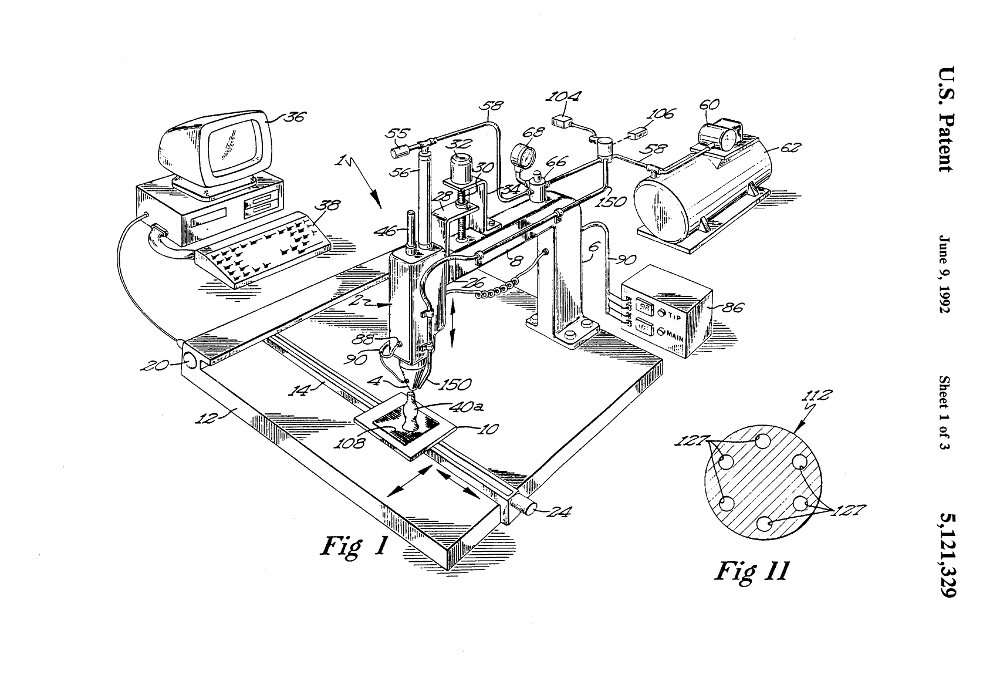
\includegraphics[width=\textwidth]{images/US5121329-1.png}
	\caption{US Patent 5121329}
	\label{img:us5121329a}
\end{figure}

\marginpar{The RepRap project works on creating general-purpose self-replicating
machines capable of printing plastic objects, and making them freely available
for the benefit of everyone.}

\noindent The surge of new cheap 3D printers -- as an affordable alternative to
the large, expensive industrial-grade machines -- was largely due to an
increasing number of enthusiasts from the \emph{Hacker-} and
\emph{Maker-}communities that worked on projects like the
RepRap\footnote{\url{http://reprap.org/wiki/RepRap}}, a very successful and
influential project.

As Erik De Bruijn, founder of the successful
Ultimaker\footnote{\url{https://www.ultimaker.com/}} company, discusses in his
Master's thesis \textit{``On the viability of the Open Source Development model
for the design of physical objects -- Lessons learned from the RepRap project''}
\cite{bruijn:2010}, the Open Source development model has proven to be well
suited in the field of physical fabrication.

At the same time, while many of these projects were started by communities as
non commercial Open Source\footnote{\url{http://opensource.org/}} and Open
Hardware\footnote{\url{http://www.oshwa.org/}} projects, crowdfunding platforms
like Kickstarter\footnote{\url{http://www.kickstarter.com/}} and
Indiegogo\footnote{\url{http://www.indiegogo.com/}} made raising capital for new
3D printers quick and easy, something that would not have been possible 10 years
ago. This resulted in a flood of readily assembled, affordable 3D printers even
for people lacking the skills to build their own machine from a list of parts.

%----------------------------------------------------------------------------------------

\section{From Data to Tangible Objects}

With the rapid and constantly accelerating developments in the field of 3D
printing, visualizing data as real, tangible objects has become feasible. There
are still some hurdles though.  The majority of people -- even those owning a 3D
printer -- have no experience with 3D modeling software. Most freely available
software tools to create 3D models -- like
OpenSCAD\footnote{\url{http://www.openscad.org/}} or
Blender\footnote{\url{http://www.blender.org/}} -- require a steep learning
curve and demand a nontrivial amount of learning time to create the desired
models. And platforms like
Thingiverse\footnote{\url{http://www.thingiverse.com/}} or
YouMagine\footnote{\url{https://www.youmagine.com/}} provide so many freely
available models that creating own objects is often not even a necessity.

Another aspect is that these general-purpose modeling tools are not optimized
for data visualization. Each type of visualization has to be created manually,
and when the data changes it's a lot of manual work to update the model.

\tangible{} was created to fill that void. It makes creation of customized,
printable data visualizations as 3D models easy, while at the same time
retaining a lot of flexibility for customization.

% Chapter 2

\chapter{Goals}

\label{ch:goals}

The goals of this thesis can be summarized as follows:

%----------------------------------------------------------------------------------------

\section{Features}

\begin{itemize}
	\item The result of the thesis is a Python library to visualize data as
		printable 3D objects. It should handle single- and multi-dimensional data.
	\item The library should provide a set of basic predefined shapes.
	\item It should be possible to create custom shapes using the provided
		primitives.
	\item The input and output should be decoupled. The library should act as a
		cross compiler. It should be possible to generate code for different
		backends.
	\item During the time of this thesis, the main targeted backend is
		OpenSCAD\footnote{\url{http://www.openscad.org/}}.
	\item The library should run on Python 2.7.
\end{itemize}

%----------------------------------------------------------------------------------------

\section{Usability}

\begin{itemize}
	\item The library should be
		pythonic\footnote{\url{http://stackoverflow.com/q/58968}} and easy to use.
	\item Comprehensive documentation should be available.
\end{itemize}

%----------------------------------------------------------------------------------------

\section{Quality}

\begin{itemize}
	\item The library should be well tested (at least 80\% test coverage).
	\item Tests should run automatically every time code is pushed to the
		repository.
	\item Change in test coverage should be measured each time the tests are run.
\end{itemize}

%----------------------------------------------------------------------------------------


\cleardoublepage % Empty page before the start of the next part

%------------------------------------------------

\ctparttext{What is \tangible{} about? What can it do? How is it structured?
Where could it be improved?}

\part{The Library}

% Chapter 3

\chapter{Features {\&} Usage}

\label{ch:features}

%----------------------------------------------------------------------------------------

\section{Introduction}\label{sec:features:introduction}

\tangible{} is a Python library to convert data into tangible 3D models. It
generates code for different backends. It is inspired by projects like OpenSCAD
and d3.js\footnote{\url{http://d3js.org/}}.

The Python programming language has proven to be an easy, accessible and at the
same time very powerful language for data analysis and many other tasks. Due to
its readable syntax, it's very easy to get started with it, even for people
without any prior programming knowledge.  \tangible{} tries to built upon this
foundation, by providing an easy to use software library that has ``batteries
included''. It should be easy to process a dataset, normalize the values and
generate the desired visualization.

The difference from Projects like
SolidPython\footnote{\url{https://github.com/SolidCode/SolidPython}} is that
\tangible{} is a modular system with an intermediate representation of objects
that is capable of generating code for different backends, it's not tied to a
single representation. Additionally, its main focus is not general CAD, but
printable 3D visualization of data.

Besides the support for model generation and different backends, \tangible{}
also provides utilities to preprocess data, e.g. for normalization of data or
for grouping and aggregation of data.

The library runs on Python 2.6 and 2.7. Support for Python 3.3+ is planned.

%----------------------------------------------------------------------------------------

\section{Usage}\label{sec:features:usage}

\tangible{} was designed to be very straightforward to use. Common data
visualizations should be possible with just a few lines of code.

Visualizing data with \tangible{} consists of three steps: Preprocessing the
data, creating a shape instance and finally rendering the code using the desired
backend.

\subsection{Preprocessing Data}

Many times the data is not yet in the right form for visualization. Let's say
that the user has air temperature measurements for every hour during an entire
day. The temperature range is between 8\si{\degree}C during the night and
22\si{\degree}C during the day.

\vspace{.5\baselineskip}
\begin{pythoncode}
>>> temperatures = [
>>>     10, 9, 8, 8, 9, 8, 9, 10, 12, 15, 17, 19,
>>>     20, 22, 22, 21, 20, 17, 14, 12, 11, 10, 9, 10
>>> ]
\end{pythoncode}

\noindent To visualize the data, the user wants to create a round tower where
the radius of a slice corresponds to a temperature measurement. But the
temperatures are not well suited to be used directly as millimeter values.
Therefore the user wants to linearly transform the range 8--22 (\si{\degree}C)
to the range 10--40 (mm).

\tangible{} provides helper functions for this called \emph{scales}. First a
linear scale needs to be constructed:

\vspace{.5\baselineskip}
\begin{pythoncode}
>>> from tangible import scales
>>> scale = scales.linear(domain=[8, 22], codomain=[10, 40])
\end{pythoncode}

\noindent The returned object is the actual scaling function. It can be used directly:

\vspace{.5\baselineskip}
\begin{pythoncode}
>>> scale(8)
10.0
>>> scale(15)
25.0
>>> scale(22)
40.0
\end{pythoncode}

\noindent ...or it can be used in combination with Python's \texttt{map()}
function:

\vspace{.5\baselineskip}
\begin{pythoncode}
>>> radii = map(scale, temperatures)
>>> radii
[14.285714285714285, 12.142857142857142, 10.0, 10.0, ...]
\end{pythoncode}

\noindent Now the data is ready to be visualized. There are also several other
functions to preprocess data, for example to group or aggregate datapoints. For
more information, take a look at section \ref{sec:architecture:utils}
\hyperref[sec:architecture:utils]{Utils}.

\subsection{Creating a Shape Instance}

\tangible{} provides many predefined shapes that can be used directly. Currently
there are three types of shapes: Vertical shapes, bar shapes and pie shapes.

For the temperature tower, the user needs the \texttt{CircleTower1D} shape from
the \texttt{tangible.shapes.vertical} module. The class requires two arguments:
The data list as well as the height of each layer.

\vspace{.5\baselineskip}
\begin{pythoncode}
>>> from tangible.shapes.vertical import CircleTower1D
>>> tower = CircleTower1D(data=radii, layer_height=2)
\end{pythoncode}

\noindent An overview over all shape classes can be found in section
\ref{subsec:architecture:shapes:classes}.

\subsection{Rendering the Code}

Now the shape is ready to be rendered. First, choose the desired backend from
the \texttt{tangible.backends} package. At the time of this writing, the only
available backend is the OpenSCAD backend.

\vspace{.5\baselineskip}
\begin{pythoncode}
>>> from tangible.backends.openscad import OpenScadBackend
\end{pythoncode}

\noindent Next, render the shape using this backend. For convenience, we write
the resulting code directly into a file.

\vspace{.5\baselineskip}
\begin{pythoncode}
>>> with open('tower.scad', 'w') as f:
...     code = tower.render(backend=openscad.OpenScadBackend)
...     f.write(code)
\end{pythoncode}

\noindent The OpenSCAD code can now be rendered on the command line (or
alternatively from the GUI tool) into an image for previewing or into an STL
file for printing:

\vspace{.5\baselineskip}
\begin{minted}[bgcolor=tango-bg,frame=lines,framesep=2mm,samepage=true,fontsize=\footnotesize]{bash}
$ openscad -o tower.png --render --imgsize=512,512 tower.scad
CGAL Cache insert: cylinder($fn=0,$fa=12,$fs=2,h=5,r1=14.28)
CGAL Cache insert: cylinder($fn=0,$fa=12,$fs=2,h=5,r1=12.14)
...
$ openscad -o tower.stl --render tower.scad
CGAL Cache insert: cylinder($fn=0,$fa=12,$fs=2,h=5,r1=14.28)
CGAL Cache insert: cylinder($fn=0,$fa=12,$fs=2,h=5,r1=12.14)
...
\end{minted}

\noindent The result:

\begin{figure}[H]
	\centering
	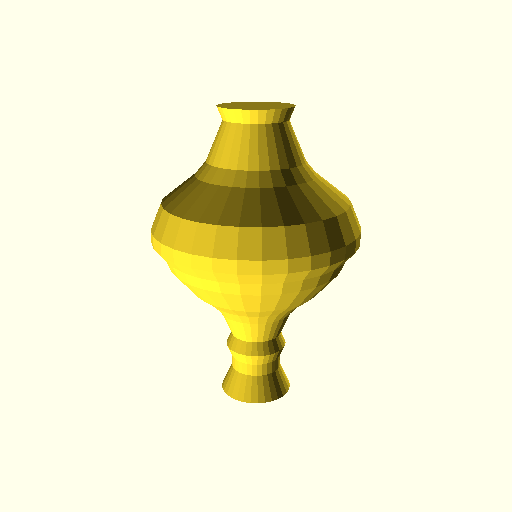
\includegraphics[height=.28\textheight]{images/usage_tower.png}
	\caption{3D visualization of a temperature range}
	\label{img:usage_tower}
\end{figure}

\noindent A few more usage examples are available in the
\hyperref[ch:examples]{\emph{Examples}} chapter on page \pageref{ch:examples}.

%----------------------------------------------------------------------------------------

\section{Future Developments}\label{sec:features:future}

There are many areas where \tangible{} could still be improved, for example by
adding more backends and shapes, by improving Python version support or by
adding more utils and helper functions.

\subsection{More Backends}

OpenSCAD was chosen as the initial backend because of its popularity. Moreover,
it's freely available and open source. Due to its programmatic nature, it's easy
to implement as a backend and it also allows the resulting code to be modified
directly to make some final adjustments before printing.

Another possible backend would have been
ImplicitCAD\footnote{\url{http://www.implicitcad.org/}}. It's a project strongly
inspired by OpenSCAD but with additional features on top of it. ImplicitCAD is is
written in Haskell and supports both an OpenSCAD compatible "legacy" syntax as
well as the traditional Haskell notation.

Both of these examples are programmatic CAD tools. A step further would be to
support the widely used STL format directly as a backend. But implementing
direct STL generation would have gone beyond the scope of this thesis and was
therefore not attempted.

\subsection{More Shapes}

Right now \tangible{} provides three base shape types with different variants.
But the shape library could be further extended, in order to provide even more
visualizations that can be used by users without any additional modeling
efforts.

\subsection{Interpolation / Smoothing}

\tangible{} provides no tools for interpolation / smoothing of surfaces. This
means that shapes with a lot of datapoints may look very ragged and printing
them may cause problems because of the overhanging surfaces.

Although libraries like Numpy\footnote{\url{http://www.numpy.org/}} and
SciPy\footnote{\url{http://www.scipy.org/}} provide interpolation functionality,
this is something that \tangible{} should provide out of the box. A possible way
of implementing curve smoothing would be by using spline interpolation. This
feature is planned for a future release.

\subsection{Data Preprocessing Tools}

The current selection of data preprocessing tools is already very useful, but
still doesn't cover many use cases. Therefore these utils should be expanded,
for example by adding logarithmic and exponential scales and by adding more
grouping functions. Furthermore the scales could be improved to allow changes in
the domain / codomain as well as rescaling of the data at any point in time.

\subsection{Python 3 Support}

Right now \tangible{} is written for Python 2.6/2.7. But it would be quite easy
to add support for Python 3.3+, especially because the extensive use of future
imports (see section \ref{sec:development:futures}). Python 3 support is already
planned and will be implemented soon.


%----------------------------------------------------------------------------------------

% Chapter 4

\chapter{Architecture}

\label{ch:architecture}

%----------------------------------------------------------------------------------------

\section{Overview}\label{sec:architecture:overview}

\tangible{} is implemented as a single Python package, without any external
dependencies.

The architecture of \tangible{} can be categorized into four different
components: The abstract syntax tree \eqref{sec:architecture:ast}, code
generation backends \eqref{sec:architecture:backends}, shapes
\eqref{sec:architecture:shapes} and utils \eqref{sec:architecture:utils}.

\vspace{7mm}

\begin{figure}[H]
	\centering
	\definecolor{BackendsColor}{RGB}{116,143,204}
\definecolor{AstColor}{RGB}{199,108,107}
\definecolor{ShapesColor}{RGB}{227,225,107}
\definecolor{UtilsColor}{RGB}{118,219,125}

\begin{tikzpicture}

	% Main rectangles

	\filldraw [fill=BackendsColor] (0,-1.75) rectangle (8,0.5);
	\filldraw [fill=AstColor] (0,0.5) rectangle node [align=center] {AST} (8,2);
	\filldraw [fill=ShapesColor] (0,2) rectangle (4,6);
	\filldraw [fill=UtilsColor] (4,2) rectangle (8,6);

	% Inner rectangles

	\draw (0.5,2.5) rectangle node [font=\footnotesize] {Base} (3.5,3.5);
	\draw (0.5,3.5) rectangle node [rotate=90,font=\footnotesize] {Bars} (1.5,5.25);
	\draw (1.5,3.5) rectangle node [rotate=90,font=\footnotesize] {Vertical} (2.5,5.25);
	\draw (2.5,3.5) rectangle node [rotate=90,font=\footnotesize] {Pie} (3.5,5.25);

	\draw (5,2.5) rectangle node [rotate=90,font=\footnotesize] {Scales} (6,5.25);
	\draw (6,2.5) rectangle node [rotate=90,font=\footnotesize] {Helper Functions} (7,5.25);

	\draw (0.5, -1.25) rectangle node [font=\footnotesize] {OpenSCAD} (4, -0.25);
	\draw (4, -1.25) rectangle node [font=\footnotesize] {...} (7.5, -0.25);

	% Labels

	\node [below] at (2,6) {Shapes};
	\node [below] at (6,6) {Utils};
	\node [below] at (4,0.5) {Backends};

\end{tikzpicture}

	\caption{Architecture Diagram}
	\label{img:architecture}
\end{figure}

%----------------------------------------------------------------------------------------

\section{AST}\label{sec:architecture:ast}

The \texttt{ast.py} module provides the objects for the abstract syntax tree
(AST) for \tangible{}. All AST objects extend a single base class called
\texttt{AST}. This base class is responsible for three things:

\begin{itemize}
	\item It provides a single base type that can be used for type checking, e.g.
		\texttt{isinstance(mysubclass, ast.AST)}.
	\item It overrides the \texttt{\_\_eq\_\_} and \texttt{\_\_ne\_\_} methods,
		with the result that all subclasses are compared by value (using
		\texttt{self.\_\_dict\_\_}), and not by identity.
	\item It provides a \texttt{\_\_repr\_\_} implementation that displays both
		the class name as well as the object memory address, which simplifies
		debugging.
\end{itemize}

\noindent The module contains the following classes:

\subsection{Base Class}

\begin{itemize}
	\item \texttt{AST}: The base shape for all AST elements, as described above.
\end{itemize}

\subsection{2D Shapes}

\begin{itemize}
	\item \texttt{Circle}: A circle shape with a specified radius.
	\item \texttt{CircleSector}: A circle sector shape (pizza slice) with a
		specified radius and angle.
	\item \texttt{Rectangle}: A rectangular shape with a specified width and
		height.
	\item \texttt{Polygon}: A polygon shape made from a list of 2D coordinates.
\end{itemize}

\subsection{3D Shapes}

\begin{itemize}
	\item \texttt{Cube}: A cube with a specified width, height and depth.
	\item \texttt{Sphere}: A sphere with a specified radius.
	\item \texttt{Cylinder}: A cylinder with a height and top/bottom radii.
	\item \texttt{Polyhedron}: An arbitrary 3D shape made from connected triangles
		or quads.
\end{itemize}

\subsection{Transformations}

\begin{itemize}
	\item \texttt{Translate}: Used to translate an object.
	\item \texttt{Rotate}: Used to rotate an object.
	\item \texttt{Scale}: Used to scale an object.
	\item \texttt{Mirror}: Used to mirror an object.
\end{itemize}

\subsection{Boolean Operations}

\begin{itemize}
	\item \texttt{Union}: A combination of multiple shapes into a single shape.
	\item \texttt{Difference}: A boolean difference of two or more shapes.
	\item \texttt{Intersection}: A boolean intersection of two or more shapes.
\end{itemize}

\subsection{Extrusions}

\begin{itemize}
	\item \texttt{LinearExtrusion}: An extrusion of a 2D object linearly along the
		z axis.
	\item \texttt{RotateExtrusion}: An extrusion of a 2D object around the z axis. 
\end{itemize}

%----------------------------------------------------------------------------------------

\section{Backends}\label{sec:architecture:backends}

The backends are responsible for code generation. They receive an
\hyperref[sec:architecture:ast]{AST} instance, traverse it and emit backend specific code.

At the time of this writing, only one backend has been implemented: The OpenSCAD
backend. But it would be very easy to add additional backends in the future.

\subsection{Creating Custom Backends}

\marginpar{In duck typed programming languages like Python, interfaces are
usually not declared explicitly. The adherence to the interface is only judged
by the behavior of the implementation: If it looks like a duck, swims like a
duck, and quacks like a duck, then it probably is a duck.}

To be valid, a custom backend simply needs to implement the following interface:

\vspace{.5\baselineskip}
\begin{pythoncode}
class CustomBackend(object):
    def __init__(self, ast):
        """Initialize backend using the provided AST."""
    def generate(self):
        """Generate code from AST and return it
        as a unicode string."""
\end{pythoncode}

\noindent The code generated by a backend is returned as a unicode string. It
can then be printed to the terminal or used for further processing.

Implementation details regarding the already existing backend can be found in
section \ref{sec:design:codegen}.

%----------------------------------------------------------------------------------------

\section{Shapes}\label{sec:architecture:shapes}

The \texttt{shapes} package is a key component of \tangible{}. It provides a
hierarchical collection of predefined shapes that can be used directly to
generate three dimensional data visualizations.

\vspace{.5\baselineskip}

\noindent The package is organized into different files:

\begin{itemize}
	\item \texttt{base.py}: Base classes for all shape objects.
	\item \texttt{mixins.py}: Mixins used in the shape classes, mostly used for
		data validation.
	\item \texttt{bars.py}: Bar like shapes.
	\item \texttt{vertical.py}: Vertical shapes, e.g. towers.
	\item \texttt{pie.py}: Circular "pie" shapes.
\end{itemize}

\begin{figure}[H]
	\centering
	\definecolor{ShapesColor}{RGB}{227,225,107}

\begin{tikzpicture}

	% Main rectangles

	\filldraw [fill=ShapesColor] (0,0) rectangle (5,5);

	% Inner rectangles

	\draw (1.5,0.5) rectangle node {\texttt{base.py}} (4.5,1.5);
	\draw (1.5,1.5) rectangle node [rotate=90] {\texttt{bars.py}} (2.5,4.25);
	\draw (2.5,1.5) rectangle node [rotate=90] {\texttt{vertical.py}} (3.5,4.25);
	\draw (3.5,1.5) rectangle node [rotate=90] {\texttt{pie.py}} (4.5,4.25);
	\draw (0.5,0.5) rectangle node [rotate=90] {\texttt{mixins.py}} (1.5,4.25);

	% Labels

	\node [below] at (2.5,5) {\texttt{shapes/}};

\end{tikzpicture}

	\caption{Shapes Architecture}
	\label{img:shapes}
\end{figure}

\subsection{Base Class}

The class \texttt{Shape} in \texttt{shapes/base.py} is the base class for all
predefined shapes in \tangible{}:

\vspace{.5\baselineskip}

\begin{pythoncode}
class BaseShape(object):
    def _build_ast(self):
        raise NotImplementedError("_build_ast method not implemented.")

    def render(self, backend):
        ast = self._build_ast()
        return backend(ast).generate()
    
class Shape(BaseShape):
    def __init__(self, data):
        self.data = utils.ensure_list_of_lists(data)
        if len(self.data[0]) == 0:
            raise ValueError("Data may not be empty.")
\end{pythoncode}

\noindent Each shape is initialized with the data as the first positional
argument. Using a helper function, single lists with one dimensional data are
converted to nested lists, to simplify the rendering code. Empty data is not
allowed.

The \texttt{\_build\_ast()} method is not implemented in the base class. An
inheriting class needs to override the method and return an AST.

Finally, the \texttt{render(backend)} method renders the AST using the specified
backend class and returns the resulting source code as a unicode string, as
described in section \ref{sec:architecture:backends}.

\subsection{Mixins}

The mixin classes are used in combination with Python's multiple inheritance
system to provide "pluggable" generic data validation. At the time of this
writing, the following mixins are available:

\begin{itemize}
	\item \texttt{Data1DMixin}: Ensures that data contains exactly 1 dataset.
	\item \texttt{Data2DMixin}: Ensures that data contains exactly 2 datasets.
	\item \texttt{Data3DMixin}: Ensures that data contains exactly 3 datasets.
	\item \texttt{Data4DMixin}: Ensures that data contains exactly 4 datasets.
	\item \texttt{DataNDMixin}: Used for shapes where the number of data
		dimensions is not relevant. But it asserts that the data is not empty and
		that all data items are of a sequence type.
	\item \texttt{SameLengthDatasetMixin}: Ensures that all datasets have the same
		length.
\end{itemize}

\noindent The mixins are properly implemented using Python's argument list
unpacking (\texttt{\textsuperscript{*}args, \textsuperscript{**}kwargs}) and
\texttt{super()} calls, so that a class can use multiple mixins without breaking
the inheritance chain. A good example where this is used is the
\texttt{RectangleTower2D} shape:

\vspace{.5\baselineskip}

\begin{pythoncode}
class RectangleTower2D(Data2DMixin,
    SameLengthDatasetMixin, VerticalShape):
    # ...
\end{pythoncode}

\subsection{Shape Classes}\label{subsec:architecture:shapes:classes}

The final shape classes are grouped into three categories: Bar shapes, vertical
shapes and pie shapes.

\begin{itemize}
	\item Bar shapes consist of several bars that start on \texttt{z=0} and have a
		height depending on the corresponding datapoint. They can be aligned in
		rows, and rows can be combined to create 3D bar graphs.
	\item A vertical shape is a shape with layers stacked on top of each other,
		with a fixed layer height, for example a round tower where the radius of
		each layer corresponds to the datapoint.
	\item A pie shape can represent data as angle, height or radius of the
		corresponding slice. It is also possible to define an inner radius
		($\rightarrow$donut) and to explode the slices.
\end{itemize}

\noindent The naming of the shape classes follows a consistent pattern: First a
descriptive name of the shape (e.g. \texttt{RhombusTower} or
\texttt{RadiusHeightPie}), then the dimensionality of the data (e.g.
\texttt{1D}, \texttt{4D} or \texttt{ND}). A way to describe data dimensionality
in Python terms would be: \emph{\texttt{n}-dimensional data is a list containing
\texttt{n} lists}.

%----------------------------------------------------------------------------------------

\section{Utils}\label{sec:architecture:utils}

\subsection{Scales}

The module \texttt{scales.py} contains functions for mapping an input domain to
an output range (the codomain). For example it could be used to normalize
temperatures between 0\si{\degree}C and 100\si{\degree}C to values between 1 and
10. The scales are inspired by the quantitative scales in
\texttt{d3.js}\footnote{\url{https://github.com/mbostock/d3/wiki/Quantitative-Scales}}.

At the time of this writing, only a linear scale has been implemented. It
accepts three parameters: The domain, the codomain (output range), and whether
to clamp the values to the output range or not.

\vspace{.5\baselineskip}
\begin{pythoncode}
>>> from tangible import scales
>>> temperatures = [32, 60, 100, 0, 120, -50]
>>> domain = [0, 100]  # Input range
>>> codomain = [1, 10]  # Output range
>>> scale = scales.linear(domain, codomain, clamp=False)
>>> scale_clamp = scales.linear(domain, codomain=, clamp=True)
\end{pythoncode}

\noindent The returned object is the actual scaling function:

\vspace{.5\baselineskip}
\begin{pythoncode}
>>> scale(0)
1.0
>>> scale(50)
5.5
>>> scale(100)
10.0
\end{pythoncode}

\noindent A very convenient way to use scales is by applying them using the
\texttt{map()} function:

\vspace{.5\baselineskip}
\begin{pythoncode}
>>> map(scale, temperatures)
[3.88, 6.3999999999999995, 10.0, 1.0, 11.799999999999999, -3.5]
>>> map(scale_clamp, temperatures)
[3.88, 6.3999999999999995, 10.0, 1.0, 10, 1]
\end{pythoncode}

\noindent Logarithmic and exponential scales as well as dynamic resizing of
domains / codomains are currently not implemented, but will follow in the
future.

\subsection{Helper Functions}

The module \texttt{utils.py} contains different helper functions to simplify
common tasks.


\subsubsection{\texttt{pairwise(iterable)}}\label{subsec:architecture:pairwise}

\noindent This function returns a generator acting as a sliding window over an iterable.
Each item returned by the generator is a 2-tuple containing two consecutive
items from the original iterable.

\vspace{.5\baselineskip}

\noindent Example:

\vspace{.5\baselineskip}
\begin{pythoncode}
>>> from tangible import utils
>>> pairs = utils.pairwise([1, 2, 3, 4, 'a'])
>>> pairs
<itertools.izip object at 0xeea098>
>>> list(pairs)
[(1, 2), (2, 3), (3, 4), (4, 'a')]
\end{pythoncode}


\subsubsection{\texttt{reduceby(iterable, keyfunc, reducefunc, init)}}

This function combines the functionality of \texttt{itertools.groupby()} and
\texttt{reduce()}. It iterates over the iterable and aggregates the values using
the specified reduce function and init value as long as \texttt{keyfunc(item)}
returns the same value. Each time the key changes, the aggregated value is
yielded.

A possible use case could be the aggregation of website visits, grouped by
month. Example:

\vspace{.5\baselineskip}
\begin{pythoncode}
>>> from datetime import date
>>> from tangible import utils
>>> visits = [(date(2013, 1, 24), 27),
...           (date(2013, 1, 26), 4),
...           (date(2013, 2, 17), 19),
...           (date(2013, 3, 11), 23),
...           (date(2013, 3, 14), 42)]
>>> keyfunc = lambda x: x[0].month
>>> reducefunc = lambda x, y: x + y[1]
>>> groups = utils.reduceby(visits, keyfunc, reducefunc, 0)
>>> groups
<generator object reduceby at 0xedc5a0>
>>> list(groups)
[31, 19, 65]
\end{pythoncode}

\noindent The corresponding SQL statement would be:

\vspace{.5\baselineskip}
\begin{minted}[bgcolor=tango-bg,frame=lines,framesep=2mm,samepage=true,fontsize=\footnotesize]{sql}
SELECT SUM(visit_count) FROM visits GROUP BY MONTH(visit_date);
\end{minted}




\subsubsection{\texttt{connect\_2d\_shapes(shapes,layer\_distance, orientation)}}

This is quite a complex function. It connects a list of 2D shapes into a 3D
shape using the desired layer distance. The \texttt{orientation} argument
specifies, whether the shapes should be joined horizontally or vertically.

\noindent The main part of the function has separate implementations depending
on the 2D object. Circles are connected by joining cylinders, while rectangles
and polygons are connected by joining polyhedra.

\vspace{.5\baselineskip}

\noindent Example:

\vspace{.5\baselineskip}
\begin{pythoncode}
>>> from tangible import utils, ast
>>> shapes = [ast.Circle(3), ast.Circle(8), ast.Circle(5)]
>>> utils.connect_2d_shapes(shapes, layer_distance=10,
...     orientation='vertical')
<AST/Union: 21376464>
\end{pythoncode}


\subsubsection{\texttt{\_quads\_to\_triangles(quads)}}

This function converts a list of quads (4-tuples) to a list of triangles
(3-tuples). This is mostly because many backends require surface meshes to
consist of triangles, without support for quads.

\vspace{.5\baselineskip}

\noindent Example:

\vspace{.5\baselineskip}
\begin{pythoncode}
>>> from tangible import utils
>>> quads = [(0, 1, 2, 3)]
>>> utils._quads_to_triangles(quads)
[(0, 1, 2), (0, 2, 3)]
\end{pythoncode}

\noindent The function is mostly used internally. A stable API is not guaranteed.


\subsubsection{\texttt{\_ensure\_list\_of\_lists(data)}}

This function ensures that the argument is a list of lists. If it doesn't
contain lists or tuples, it is wrapped in a list and returned.

\vspace{.5\baselineskip}

\noindent Example:

\vspace{.5\baselineskip}
\begin{pythoncode}
>>> utils._ensure_list_of_lists([1, 2, 3])
[[1, 2, 3]]
>>> utils._ensure_list_of_lists([[1, 2], [3]])
[[1, 2], [3]]
\end{pythoncode}

\noindent The function is mostly used internally. A stable API is not guaranteed.

% Chapter 5

\chapter{Examples}

\label{ch:examples}

The following pages demonstrate a few code examples of how to use the
\tangible{} library.

%----------------------------------------------------------------------------------------

\section{A difficult Tower}\label{sec:tower}

I work in different file describes a simple round tower where the radius of the layers
corresponds to the datapoint. The dataset describes the number of web site
visits on \url{http://blog.dbrgn.ch/} during the month of September 2013. The
value range is normalized to a range between 10 and 50 using a linear scale.

\vspace{.5\baselineskip}
\begin{pythoncode}
from tangible import scales
from tangible.shapes.vertical import CircleTower1D
from tangible.backends.openscad import OpenScadBackend

# Normalize raw data
visits = [53, 69, 86, 92, 81, 76, 37, 36, 62, 76, 72, 67, 55, 61, 54,
          72, 92, 84, 78, 75, 45, 48, 85, 81, 83, 69, 68, 66, 62, 115]
scale = scales.linear([min(visits), max(visits)], [10, 50])
datapoints = map(scale, visits)

# Create shape
tower = CircleTower1D(datapoints, layer_height=10)

# Render OpenSCAD code
code = tower.render(backend=OpenScadBackend)
print code
\end{pythoncode}
\vspace{.5\baselineskip}

\begin{figure}[H]
	\centering
	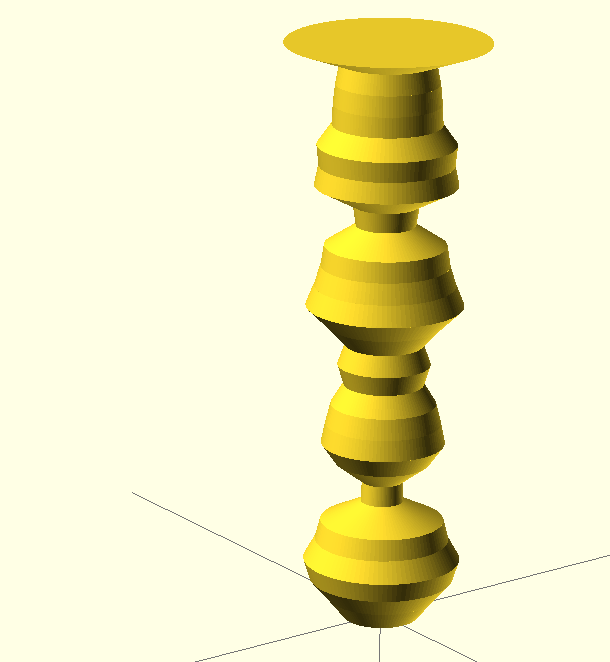
\includegraphics[height=.25\textheight]{images/tower.png}
	\caption{A CircleTower1D shape}
	\label{img:tower}
\end{figure}

%----------------------------------------------------------------------------------------

\newpage
\section{Multi Dimensional Data}\label{sec:multidimensional}

Here we have two dimensional data, represented as two lists of integers. The
first list should be mapped to the angle of the ``pie slices'', while the second
list should be mapped to the height of each slice. Additionally, we'll add a
center radius to make the model look like a donut, and we'll explode the slices.

\vspace{.5\baselineskip}
\begin{pythoncode}
from tangible.shapes.pie import AngleHeightPie2D
from tangible.backends.openscad import OpenScadBackend

# Data
datapoints = [
    [30, 30, 5, 5, 20], # Angle
    [18, 23, 20, 15, 10], # Height
]

# Create shape
pie = AngleHeightPie2D(datapoints, inner_radius=4, explode=1)

# Render OpenSCAD code
code = pie.render(backend=OpenScadBackend)
print code
\end{pythoncode}
\vspace{.5\baselineskip}

\begin{figure}[H]
	\centering
	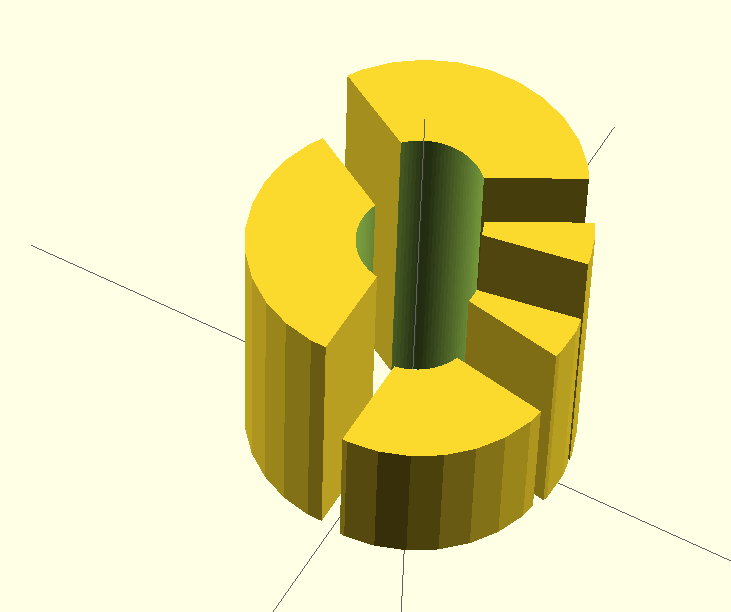
\includegraphics[height=.3\textheight]{images/angle_pie.png}
	\caption{An AnglePie2D shape}
	\label{img:angle_pie}
\end{figure}

%----------------------------------------------------------------------------------------

\newpage
\section{Reading Data from CSV}\label{sec:csv}

Often the data that you want to visualize is not already available as a Python
datastructure, but in formats like JSON or CSV. Here's a small example where
website visitor data is read from the CSV exported by Google Analytics. Then the
number of visits and the average visit duration are mapped to the distance
between opposing corners of a rhombus tower.

\vspace{.5\baselineskip}
\begin{pythoncode}
import csv
from datetime import timedelta
from tangible.shapes.vertical import RhombusTower2D
from tangible.backends.openscad import OpenScadBackend

# Read data into list
datapoints = [[], []]
with open('analytics-sep-13.csv', 'r') as datafile:
    reader = csv.DictReader(datafile)
    for row in reader:
        datapoints[0].append(int(row['Visits']))
        h, m, s = map(int, row['AvgDuration'].split(':'))
        duration = timedelta(hours=h, minutes=m, seconds=s)
        datapoints[1].append(duration.total_seconds())

# Create shape
tower = RhombusTower2D(datapoints, layer_height=10)

# Render OpenSCAD code
code = tower.render(backend=OpenScadBackend); print code
\end{pythoncode}
\vspace{.5\baselineskip}

\noindent Here are the CSV contents:

\vspace{.5\baselineskip}
\begin{minted}[frame=lines,framesep=2mm,samepage=true,fontsize=\footnotesize]{text}
Day,Visits,AvgDuration
9/1/13,53,00:00:51
9/2/13,69,00:01:01
9/3/13,86,00:01:24
...
\end{minted}
\vspace{.5\baselineskip}

\noindent And the resulting shape:

\begin{figure}[H]
	\centering
	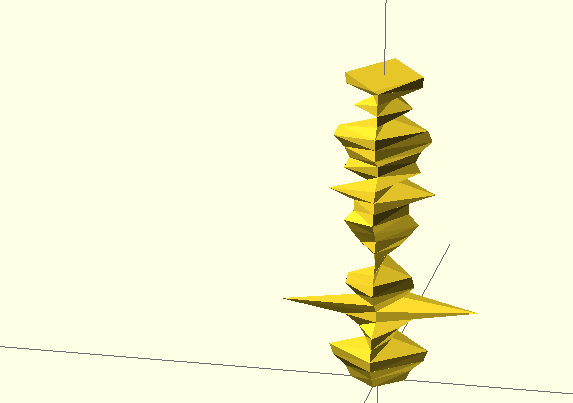
\includegraphics[height=.20\textheight]{images/csv.png}
	\caption{A RhombusTower2D shape from CSV data}
	\label{img:angle_pie}
\end{figure}


%----------------------------------------------------------------------------------------

\newpage
\section{Grouped Data}\label{sec:tower}

Some one dimensional datasets does not work well when visualized directly. An
example would be website visitor statistics during a full year, a single bar
graph would be much too wide. But by grouping the data from example
\ref{sec:csv} into months, a \texttt{BarsND} graph can be constructed:

\vspace{.5\baselineskip}
\begin{pythoncode}
import csv
from itertools import chain
from tangible import scales
from tangible.shapes.bars import BarsND
from tangible.backends.openscad import OpenScadBackend

# Read data into list
datapoints = [list() for i in xrange(9)]
with open('analytics-full-13.csv', 'r') as datafile:
    reader = csv.DictReader(datafile)
    for row in reader:
        date = row['Day']
        month = int(date.split('/', 1)[0])
        visits = int(row['Visits'])
        datapoints[month - 1].append(visits)

# Normalize data
all_datapoints = list(chain.from_iterable(datapoints))
scale = scales.linear([min(all_datapoints), max(all_datapoints)],
                      [10, 150])
datapoints = map(lambda x: map(scale, x), datapoints)

# Create shape
bars = BarsND(datapoints, bar_width=7, bar_depth=7)

# Render OpenSCAD code
code = bars.render(backend=OpenScadBackend); print code
\end{pythoncode}
\vspace{.5\baselineskip}

\begin{figure}[H]
	\centering
	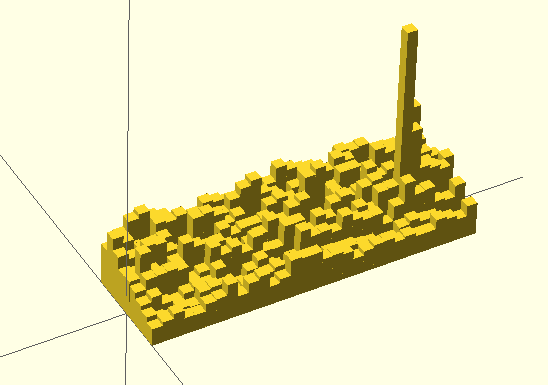
\includegraphics[height=.28\textheight]{images/bars_nd.png}
	\caption{A BarsND shape from CSV data grouped by month}
	\label{img:bars_nd}
\end{figure}

%----------------------------------------------------------------------------------------

\newpage
\section{Creating Custom Shapes from AST}\label{sec:custom_ast}

It's not necessary to rely on the provided shape classes only, you can also
create your own shapes by using the \hyperref[sec:ast]{AST} objects directly.

The easiest and cleanest way to do this, is to create a subclass of the
\texttt{BaseShape} class and to override its \texttt{\_build\_ast} method:

\vspace{.5\baselineskip}
\begin{pythoncode}
from tangible.shapes.base import BaseShape
from tangible import ast
from tangible.backends.openscad import OpenScadBackend

# Create custom shape
class Cogwheel(BaseShape):
    def _build_ast(self):
        cogs = []
        for i in xrange(18):
            cog = ast.Rectangle(2, 2)
            translated = ast.Translate(9.5, -1, 0, cog)
            rotated = ast.Rotate(i * 30, (0, 0, 1), translated)
            cogs.append(rotated)
        return ast.Union([ast.Circle(radius=10)] + cogs)

# Render shape
f = Cogwheel()
code = f.render(backend=OpenScadBackend)
print code
\end{pythoncode}
\vspace{.5\baselineskip}

\begin{figure}[H]
	\centering
	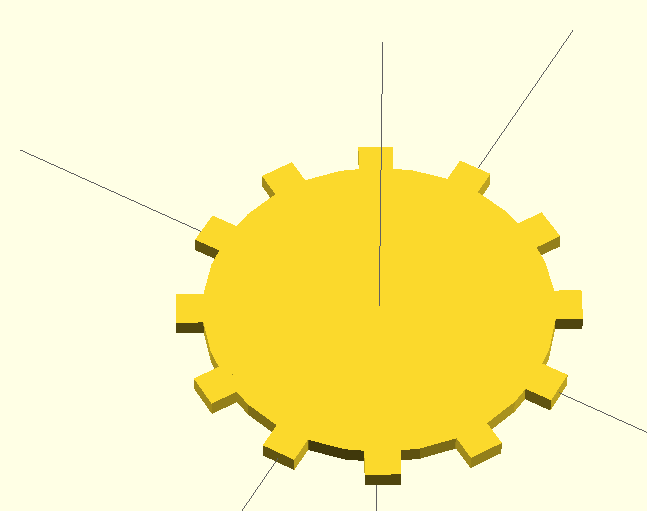
\includegraphics[height=.3\textheight]{images/cogwheel.png}
	\caption{A custom cogwheel shape}
	\label{img:cogwheel}
\end{figure}


%------------------------------------------------

\ctparttext{How was the library developed? What tools were used? What design
decisions were made?}

\part{The Development Process}

% Chapter 6

\chapter{Development Process \& Tools Used}

\label{ch:development}

%----------------------------------------------------------------------------------------

\section{Coding Guidelines}

\marginpar{The PEPs (Python Enhancement Proposals) are Python's way of
continuously improving the language in a community driven process. Any community
member can submit a proposal for a language change, which is then discussed and
accepted or rejected.}

Coding guidelines are important in order to achieve a consistent style
throughout the codebase. In the Python world, the PEP8 style guide
\cite{pep8:2001} has seen near ubiquitous adaptation and should be used for all
projects in order to aid the legibility of the source code.

\begin{quote}{\slshape
One of Guido's key insights is that code is read much more often than it is
written. The guidelines provided here are intended to improve the readability of
code and make it consistent across the wide spectrum of Python code. As PEP 20
says, ``Readability counts''. \\ \medskip
--- \defcitealias{pep8:2001}{Style Guide for Python Code}\citetalias{pep8:2001} \citep{pep8:2001}
}\end{quote}

\noindent \tangible{} follows most parts of PEP8, with two exceptions:

\begin{itemize}
	\item While line lengths below 80 characters are the ideal case, lines with up
		to 99 characters are still acceptable, if it makes the code more readable.
	\item Errors \texttt{E126--E128}, which specify indentation rules for
		multi-line statements, can be ignored.
\end{itemize}

\noindent The adherence to these coding guidelines is tested automatically by
the test suite (see section \ref{sec:development:testing}). Violations are
counted as test failures.

%----------------------------------------------------------------------------------------

\section{Future Imports}\label{sec:development:futures}

While the first version of Python 3 has been released back in 2008, it has still
not completely managed to replace the older 2.x versions. As a result, the
\tangible{} codebase currently targets Python 2.

But in the past year several things have happened that accelerated the adoption
rate of Python 3. Most importantly, several big Linux distributions like Arch
Linux\footnote{\url{https://www.archlinux.org/}} and
Fedora\footnote{\url{http://fedoraproject.org/}} have decided to move to Python
3 as the default Python implementation. Another important factor was the newly
added Python 3 support in big Python frameworks like
Django\footnote{\url{https://www.djangoproject.com/}}.

In view of these facts, the \tangible{} source code is written in a forward
compatible way by adding ``future-imports'' to the top of every code file.
Python provides a module called \texttt{future} which contains backports of
newer language features to older Python versions. By using these imports, the
migration process to newer language versions can be substantially simplified.

In the \tangible{} Project, the following preamble should be added to every
source code file:

\vspace{.5\baselineskip}
\begin{pythoncode}
# -*- coding: utf-8 -*-
from __future__ import print_function, division
from __future__ import absolute_import, unicode_literals
\end{pythoncode}

\noindent This results in the following effects:

\begin{itemize}
	\item The \texttt{\# -*- coding: utf-8 -*-} line tells the Python interpreter
		that this file source is UTF8-encoded. In Python 3 UTF8 encoding will become
		the default.
	\item The \texttt{print\_function} import removes the \texttt{print} statement
		and adds a \texttt{print()} function.
	\item When activating the \texttt{division} import, division of two integers
		results in a \texttt{float} value instead of the old, lossy way of returning
		a floored integer. When floor division is explicitly desired, the
		\texttt{//} operator should be used instead.
	\item By importing \texttt{absolute\_import}, Python prioritizes absolute
		imports over relative imports. This fixes a few issues with import name
		clashes.
	\item The \texttt{unicode\_literals} import is the one with the most
		consequences of all the future imports listed above. It changes the default
		type of strings from bytestrings to unicode objects. By eliminating this
		Python 2/3 inconsistency from the beginning, many hard to spot migration
		bugs can be prevented.
\end{itemize}

\noindent The choice of future imports is based on the article \emph{Quick Tips
on Making Your Code Python 3 Ready} by Hristo Deshev \cite{deshev:2012}.

%----------------------------------------------------------------------------------------

\section{Testing} \label{sec:development:testing}

\begin{quote}{\slshape
More than the act of testing, the act of designing tests is one of the best bug
preventers known. The thinking that must be done to create a useful test can
discover and eliminate bugs before they are coded — indeed, test-design thinking
can discover and eliminate bugs at every stage in the creation of software, from
conception to specification, to design, coding and the rest.\\ \medskip
--- \defcitealias{beizer:2003}{Boris Beizer}\citetalias{beizer:2003} \citep{beizer:2003}
}\end{quote}

\marginpar{\vspace{2\baselineskip}\\Test Driven Development (TDD) is a software
development methodology where tests are written for every feature before it is
implemented.}

\noindent Testing is not a question of "whether", but rather a question of
"how". By having a high test coverage of your code base, code can be changed
without any fear of overlooking newly introduced bugs. Additionally, the TDD
methodology greatly aids both the process of writing tests, as well as the
process of writing software. Writing tests before actually implementing the code
leads to better structured code with less bugs than if testing features after
their implementation.

This section can be divided into three subsections: Writing the tests, running
the tests and measuring test coverage.

\subsection{Writing Tests}

\tangible{} uses the pytest\footnote{\url{http://pytest.org/}} framework for
writing tests. pytest provides both tools for easy and lightweight testing as
well as a simple method for test discovery.

In contrast to Python's builtin \texttt{unittest} module, which was heavily
inspired by Java, pytest does not require the developer to use explicit methods
for expressing assertions like \texttt{assertEquals} or \texttt{assertGreater}.
Instead it relies solely on the \texttt{assert} keyword while still providing
useful error messages by using language reflection.

A simple test could just look like the following example:

\vspace{.5\baselineskip}
\begin{pythoncode}
def test_the_answer():
    assert 19 + 23 == 42
\end{pythoncode}

\noindent In contrast, the \texttt{unittest} version would look like this:

\vspace{.5\baselineskip}
\begin{pythoncode}
import unittest
class TestTheAnswer(unittest.TestCase):
    def testIt(self):
        self.assertEquals(19 + 23, 42)
\end{pythoncode}

\noindent As the Zen of Python \cite{pep20:2004} states, \emph{``Simple is
better than complex.''}. In this regard pytest seems to be a big improvement
over the \texttt{unittest}. But simpler asserts are not the only advantage that
pytest offers over unittest.  Another feature that has been used extensively in
\tangible{} is parametrized testing. By specifying a set of possible values for
the test parameters using the \texttt{pytest.mark.parametrize} decorator,
multiple tests are generated from a single test function. If one of five input
values makes the test fail, the test result would be 4 successful tests out of a
total of 5, whereas putting all the values in a nonparametrized function would
lead to a single failing test.

Here is an example of a parametrized test from the \tangible{} test suite:

\vspace{.5\baselineskip}
\begin{pythoncode}
import pytest
from tangible import scales

@pytest.mark.parametrize(('param', 'clamp', 'expected'), [
    (2, False, 10),
    (3.5, False, 17.5),
    (6, False, 30),
    (6, True, 20),
])
def test_linear(param, clamp, expected):
    domain, codomain = (2, 4), (10, 20)
    scale = scales.linear(domain, codomain, clamp)
    assert scale(param) == expected
\end{pythoncode}


\subsection{Running Tests}

pytest offers highly customizable test discovery out of the box. After
configuring the patterns to be used for detecting tests, the suite can be run
by simply issueing \texttt{py.test} in the main project directory.

But manually running tests is a step that's often forgotten while developing.
Tests are better when they're fully automated. Travis CI
(\url{https://travis-ci.org/}) is a startup company that offers free continuous
integration for open source projects. A minimal configuration file is all that's
needed to get everything up and running. The test results are presented in an
easy to understand manner in the web browser:

\begin{figure}[H]
	\centering
	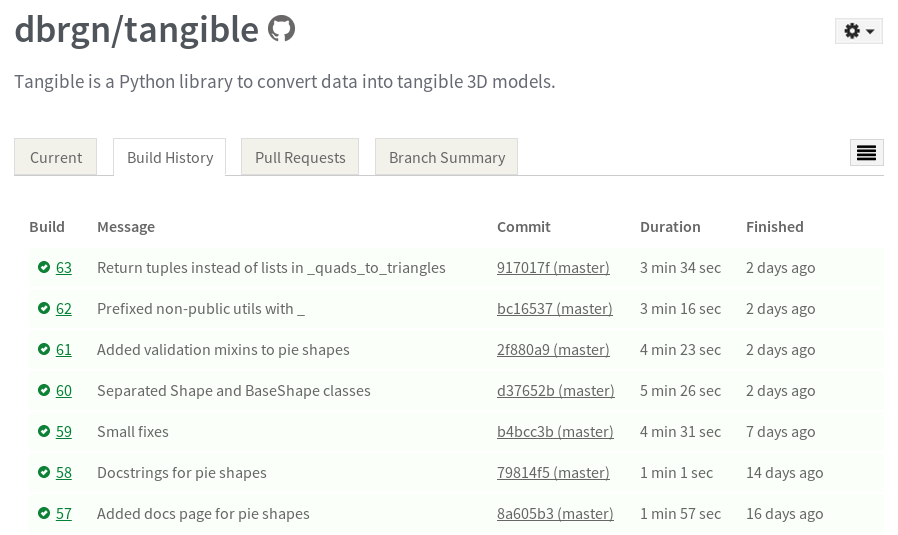
\includegraphics[width=\textwidth]{images/travis.png}
	\caption{Travis CI}
	\label{img:travis}
\end{figure}

\subsection{Measuring Test Coverage}

Simply having many tests does not necessarily mean that the code is well tested.
A high test coverage does not either, but it's a good indicator on how many
lines of code have been hit by the tests, and how many haven't.

In the \tangible{} project, coverage is measured through the
coverage.py\footnote{\url{http://nedbatchelder.com/code/coverage/}} module. The
result is displayed each time the test suite runs thanks to the
pytest-cov\footnote{\url{https://pypi.python.org/pypi/pytest-cov}} plugin for
pytest.

Change in test coverage is tracked by the Coveralls service
(\url{https://coveralls.io/}). The current coverage percentage can be displayed
in the README file by embedding a dynamic image from the Coveralls server. This
way, the current coverage is always visible.

%----------------------------------------------------------------------------------------

\section{Tools Used}

During the time of this thesis, the following tools have been used:

\begin{itemize}
	\item The Vim text editor for editing both program source code and
		documentation.\\ \url{http://www.vim.org/}
	\item Flake8 for code style checks and static code analysis.\\
		\url{https://flake8.readthedocs.org/}
	\item pytest for running the test suite.\\
		\url{http://pytest.org/}
	\item Travis CI for automated testing.\\
		\url{https://travis-ci.org/}
	\item Coveralls for automated test coverage measuring.\\
		\url{https://coveralls.io/}
	\item OpenSCAD to convert the generated model code to actual STL files.\\
		\url{http://www.openscad.org/}
	\item Makerbot / Makerware to test-print a few of the generated 3D models.\\
		\url{http://www.makerbot.com/makerware/}
	\item \LaTeX{} for typesetting this project documentation.\\
		\url{http://www.latex-project.org/}
	\item Sphinx for generating the online user documentation.\\
		\url{http://sphinx-doc.org/}
	\item Git and Github for version control.\\
		\url{http://git-scm.com/}\\
		\url{https://github.com/}
\end{itemize}

% Chapter 7

\chapter{Design Decisions \& Implementation Details}

\label{ch:design}

%----------------------------------------------------------------------------------------

\section{Pairwise Iterator} \label{sec:design:pairwise}

The pairwise iterator (in \texttt{tangible/utils.py}, see section
\ref{subsec:architecture:pairwise}) has an interesting implementation that might
not be immediately obvious to someone new to Python and its standard library:

\vspace{.5\baselineskip}
\begin{pythoncode}
from itertools import tee, izip

def pairwise(iterable):
    a, b = tee(iterable)
    next(b, None)
    return izip(a, b)
\end{pythoncode}

\noindent The \texttt{tee(iterable, n)} function returns \texttt{n} independent
iterators from a single iterable. The default value for \texttt{n} is
\texttt{2}, so in the example above two iterators called \texttt{a} and
\texttt{b} are created from the original iterable.

The second iterator is then advanced once by applying the \texttt{next()}
function to it. The return value is discarded. This results in two iterators,
one of them with an offset of 1.

As a last step, the two iterators are zipped together. By using the
\texttt{izip()} function instead of the regular \texttt{zip()}, a lazy generator
is returned instead of a list. This decreases memory consumption, especially
when handling large lists.

Now each time the returned generator is advanced one step, the sliding window is
shifted by 1 position and the resulting tuple is returned, until the end of the
iterator is reached.

\vspace{.5\baselineskip}
\begin{pythoncode}
>>> data = [1, 2, 3, 'a']
>>> pairs = pairwise(data)
>>> pairs
<itertools.izip object at 0x151def0>
>>> next(pairs)
(1, 2)
>>> next(pairs)
(2, 3)
>>> next(pairs)
(3, 'a')
>>> next(pairs)
Traceback (most recent call last):
  File "<stdin>", line 1, in <module>
	StopIteration
\end{pythoncode}

%----------------------------------------------------------------------------------------

\section{Code Generation} \label{sec:design:codegen}

Code generating code is often something quite messy, with many conditionals and
a lot of \texttt{print} statements and string formatting. Such an approach is
both hard to read and hard to maintain. Additionally, it does not reflect the
structure of the generated code.

In the OpenSCAD backend implementation, \tangible{} uses an approach proposed by
Tomer Filiba \cite{filiba:2012}, which builds upon Python's context managers to
generate nested blocks of code.

\marginpar{Context Managers are Python constructs that create a runtime context
for a piece of code when used in combination with the \texttt{with} statement.
They provide enter- and exit-hooks that are invoked before and after executing
that code.}

There is a top level class called \texttt{Program} which exposes a
\texttt{statement} method and a \texttt{block} context manager. The class holds
a stack of blocks and a list of child blocks and statements. Each time a block
is entered (by using a \texttt{with}-statement), it is pushed to the stack and
appended to the list of children. When leaving the context manager, the block is
removed again from the stack.

The final code is generated by walking the list of children in the
\texttt{Program} instance recursively. This is also the point where
language-specific features can be implemented, for example indentation of a
block in Python or inserting curly braces in Java or C.

A special feature that was implemented in the code generation is the support for
predefined code snippets to be included in the generated output. This part of
the code is called the ``preamble''. Snippets can be inserted into the preamble
multiple times, but they're rendered only once. This has proven to be very
useful while implementing code generation for circle sectors (see section
\ref{sec:design:circlesectors}).

Right now all the described classes are contained in the OpenSCAD backend. By
generalizing the code, it would be possible to create a base class for all code
generation backends, with the possibility to configure the language-specific
details in a single subclass. This might be a good idea for a future version of
\tangible{}.

An extract from the actual code which decides how the AST is mapped to the
backend syntax is shown on the next page.

\vspace{.5\baselineskip}
\begin{pythoncode}
class OpenScadBackend(object):
    """Render AST to OpenSCAD source code."""

    def __init__(self, ast):
        self.ast = ast

    def generate(self):
        prgm = Program()
        BLOCK = prgm.block
        STMT = prgm.statement
        PRE = prgm.preamble
        SEP = prgm.emptyline

        def _generate(node):
            """Recursive code generating function."""

            istype = lambda t: node.__class__ is t

            # Handle lists
            if istype(list):
                for item in node:
                    _generate(item)

            # Simple statements
            elif istype(ast.Circle):
                STMT('circle({0})', node.radius)
            elif istype(ast.Rectangle):
                STMT('square([{0}, {1}])', node.width, node.height)

            # Blocks
            elif istype(ast.Union):
                with BLOCK('union()'):
                    _generate(node.items)

            # (...)

        _generate(self.ast)

        return prgm.render()
\end{pythoncode}

%----------------------------------------------------------------------------------------

\newpage
\section{Circle Sectors in OpenSCAD}\label{sec:design:circlesectors}

By default, OpenSCAD does not support circle sectors. Therefore the shape had to
be developed manually as a module.

\vspace{.5\baselineskip}
\begin{minted}[frame=lines,framesep=2mm,samepage=true,fontsize=\footnotesize]{javascript}
module circle_sector(r, a) {
    a1 = a % 360; a2 = 360 - (a % 360);
    if (a1 <= 180) {
        intersection() {
            circle(r);
            polygon([
                [0,0],
                [0,r],
                [sin(a1/2)*r, r + cos(a1/2)*r],
                [sin(a1)*r + sin(a1/2)*r, cos(a1)*r + cos(a1/2)*r],
                [sin(a1)*r, cos(a1)*r],
            ]);
        }
    } else {
        difference() {
            circle(r);
            mirror([1,0]) {
                polygon([
                    [0,0],
                    [0,r],
                    [sin(a2/2)*r, r + cos(a2/2)*r],
                    [sin(a2)*r + sin(a2/2)*r, cos(a2)*r + cos(a2/2)*r],
                    [sin(a2)*r, cos(a2)*r],
                ]);
            };
        }
    }
};
\end{minted}

\noindent The base concept is a boolean combination of a circle and a polygon,
depending on the angle. If the angle is less than or equal to 180\si{\degree},
the resulting shape is the intersection of the circle and the polygon. If it's
larger than 180\si{\degree}, the difference between the two shapes is returned.

The polygon always consists of five points, which are calculated as shown in the
following table for angles less or equal to 180\si{\degree}. For angles between
180\si{\degree} and 360\si{\degree}, the polygon is simply mirrored along the y
axis.

\begin{table}[H]
	\centering
	\begin{tabularx}{\textwidth}{XX} \toprule
		\tableheadline{x} & \tableheadline{y} \\
		\midrule
		$0$ & $0$ \\
		$0$ & $r$ \\
		$\sin(\alpha / 2) \cdot r$ & $r + \cos(\alpha / 2) \cdot r$ \\
		$\sin(\alpha) \cdot r + \sin(\alpha / 2) \cdot r$ & $\cos(\alpha) \cdot r + \cos(\alpha / 2) \cdot r$ \\
		$\sin(\alpha) \cdot r$ & $\cos(\alpha) \cdot r$ \\
		\bottomrule
	\end{tabularx}
\end{table}

\noindent The following six images show the circle and polygon combinations for
45, 90, 180, 225, 270 and 315 degrees.

\begin{figure}[H]
	\centering
	\subfloat[]{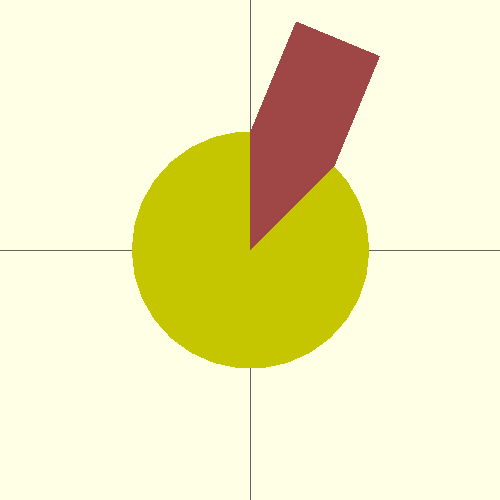
\includegraphics[width=.30\textwidth]{images/cs_45}}
	\quad
	\subfloat[]{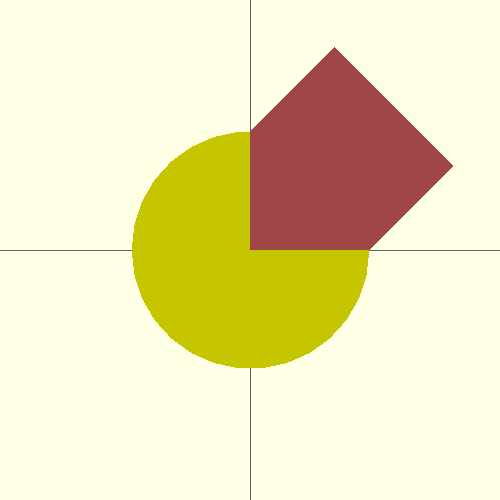
\includegraphics[width=.30\textwidth]{images/cs_90}}
	\quad
	\subfloat[]{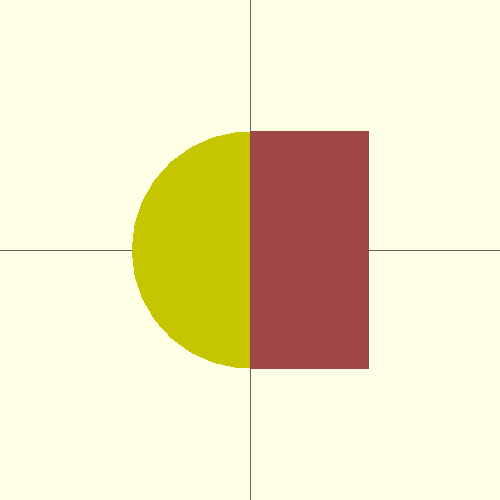
\includegraphics[width=.30\textwidth]{images/cs_180}}
	\\
	\subfloat[]{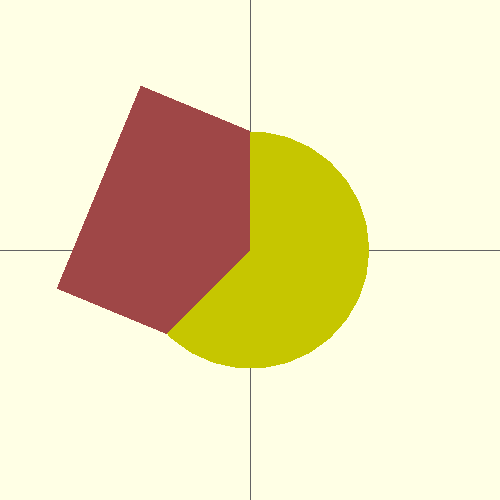
\includegraphics[width=.30\textwidth]{images/cs_225}}
	\quad
	\subfloat[]{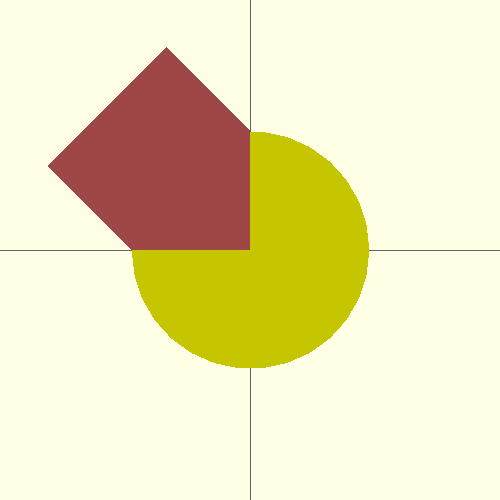
\includegraphics[width=.30\textwidth]{images/cs_270}}
	\quad
	\subfloat[]{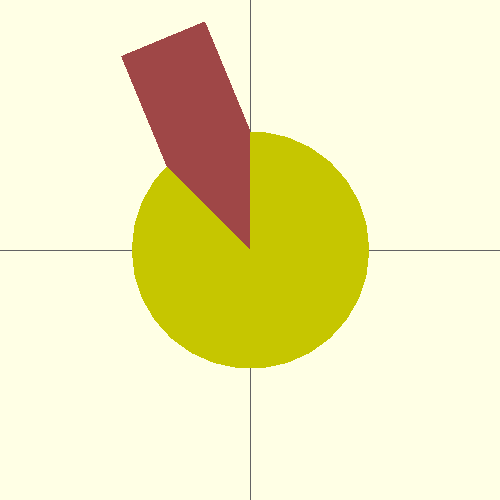
\includegraphics[width=.30\textwidth]{images/cs_315}}

	\caption{Circle and polygon combinations at different angles}
	\label{img:circle_shape_angles}
\end{figure}

\noindent By combining the two shapes in such a way, any circle sector can be
created. Example for \texttt{circle\_sector(10, 225)}:

\begin{figure}[H]
	\centering
	
\includegraphics[width=.70\textwidth]{images/cs_225_result}
	\caption{The resulting circle sector for an angle of 225\si{\degree}}
	\label{img:circle_shape_result}
\end{figure}

\noindent The module source code is used in the OpenSCAD backend implementation
as a preamble snippet.


%----------------------------------------------------------------------------------------
%	THESIS CONTENT - APPENDICES
%----------------------------------------------------------------------------------------

\appendix

\part{Appendix} % New part of the thesis for the appendix

%\include{chapters/0A} % Appendix A
%\include{chapters/0B} % Appendix B - empty template

%----------------------------------------------------------------------------------------
%	POST-CONTENT THESIS PAGES
%----------------------------------------------------------------------------------------

\cleardoublepage% Bibliography

\label{app:bibliography} % Reference the bibliography elsewhere with \autoref{app:bibliography}
\raggedright
\manualmark
\markboth{\spacedlowsmallcaps{\bibname}}{\spacedlowsmallcaps{\bibname}} 
\refstepcounter{dummy}

\addtocontents{toc}{\protect\vspace{\beforebibskip}} % Place the bibliography slightly below the rest of the document content in the table of contents
\addcontentsline{toc}{chapter}{\tocEntry{\bibname}}

\bibliographystyle{plainnat}
\bibliography{bibliography}
 % Bibliography

\cleardoublepage% Declaration

\refstepcounter{dummy}
\pdfbookmark[0]{Declaration}{declaration} % Bookmark name visible in a PDF viewer

\chapter*{Declaration} % Declaration section text

\thispagestyle{empty}

Hereby we acknowledge,

\begin{itemize}
		\item that we conducted this thesis by ourselves and without any external help,
			except with those, which are explicitly mentioned,
		\item that all used sources are cited academically correct, and 
		\item that I didn't use any copyright protected materials (e.g. images) in
			an unauthorized manner.
\end{itemize}

\bigskip
 
\noindent\textit{\myLocation, \myTime}

\bigskip

\begin{flushright}
    \begin{tabular}{m{8cm}}
    \hspace{1cm}
\includegraphics[width=.5\textwidth]{images/signature_lukas.jpg}
    \\ \hline
    \centering Lukas Martinelli, \today \\
    \end{tabular}
\end{flushright}

\begin{flushright}
    \begin{tabular}{m{8cm}}
    \hspace{2cm}
\includegraphics[width=.33\textwidth]{images/signature_manuel.png}
    \\ \hline
    \centering Manuel Roth, \today \\
    \end{tabular}
\end{flushright}


 % Declaration

%----------------------------------------------------------------------------------------

\end{document}
